\section{Modulationsarten}
Modulationsverfahren sind ein großes Anwendungsgebiet in der Nachrichtentechnik.
Ziel ist es viele Informationen Verlustfrei zu übertragen.
Möchte man ein Datensignal übertragen muss es davor
aufbereitet werden. Dies erledigt der Modulator/Mischer.
\\
Es gibt Analoge und Digitale Modulationsarten.
Für Analoge Signale werden folgende Verfahren verwendet.


\subsection{Amplitudenmodulation AM}
Die Idee hinter der Amplitudenmodulation ist dass das Informationssignal
auf die Amplitude des Trägersignals zu modulieren.
Daduch veränder sich die Amplituder des Trägersignals in abhängigkeit des Pegels und 
Freqeuenz des Informationssignals.
\\
\begin{figure}[h]
    \centering
    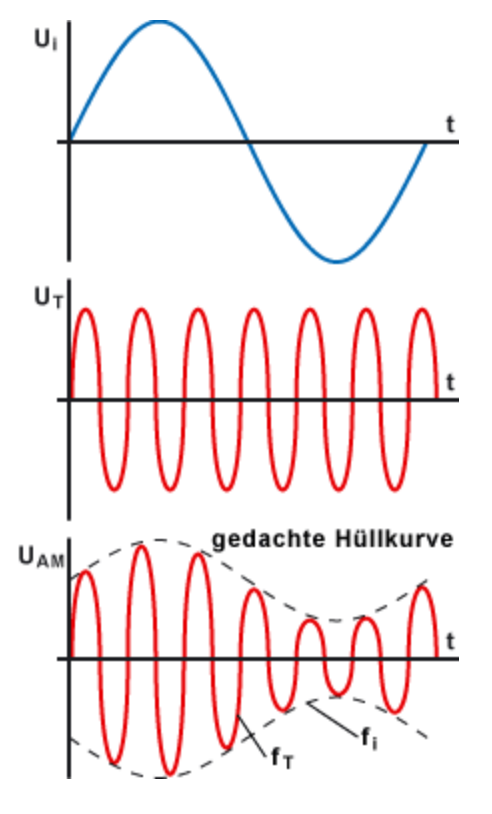
\includegraphics[width=0.22\textwidth]{Pictures/Screenshot 2025-06-19 125508.png}
    \caption{Amplitudenmodulation}
    \footnotesize{Quelle: \url{https://www.elektronik-kompendium.de/sites/kom/0401181.htm}}
    \label{fig:link_budget}
\end{figure}
\clearpage
Die Amplitude der Trägerschwingung wird durch das analoge Datensignal
$x(t)$ folgendermaßen verändert.
\begin{equation}
    a(t)=A_c(1+\mu x(t))
\end{equation}
Das AM-Signal wird beschrieben durch.
\begin{equation}
    x_c(t)=A_c(1+\mu x(t))cos(2\pi f_c t)
\end{equation}
\begin{itemize}
    \item $A_c$: Trägeramplitude
    \item $f_c$: Trägerfrequenz
    \item $\mu$: Modulationsindex 0 < $\mu$ < 1
\end{itemize}


\subsection{Frequenzmodulation FM}
Die Frequenzmodulation spielt eine eben so wichtige Rolle wie die Amplitudenmodulation,
ist im vergleich jedoch weniger Störanfällig. 
Hier wird auch ein hochfrequentes Trägersignal erzeugt und dadurch die Sendefrequenz um ein kleinen Betrag verändert.
Am einfachsten ist so eine Modulation durch ein LC-Schwingkreis.

\begin{equation}
x_c(t) = A_c \cos\left( 2\pi f_c t + 2\pi f_\Delta \int_0^t x(\tau) \, \mathrm{d}\tau \right)
\end{equation}
\begin{itemize}
    \item $x(\tau)$: Datensignal
    \item $A_c$: Amplitude des Trägersignals (konstant)
    \item $f_c$: Trägerfrequenz 
    \item $f_\Delta$: Frequenzhub, legt die maximale abwichung zu $f_c$ fest
\end{itemize}
\clearpage

\subsection{Phasenmodulation PM}
Die Phasenmodulation gehört wie die Frequenzmodulation zu den Winkelmodulationen.
Hier wird die Phase der Trägerwelle in Abhängigkeit des Datensignals verändert.
Die Phasenveränder bleibt im Signal erhalten variiert jedoch im vergleich
zur Ursprünglichen Phase des Trägersignal
\begin{figure}[h]
    \centering
    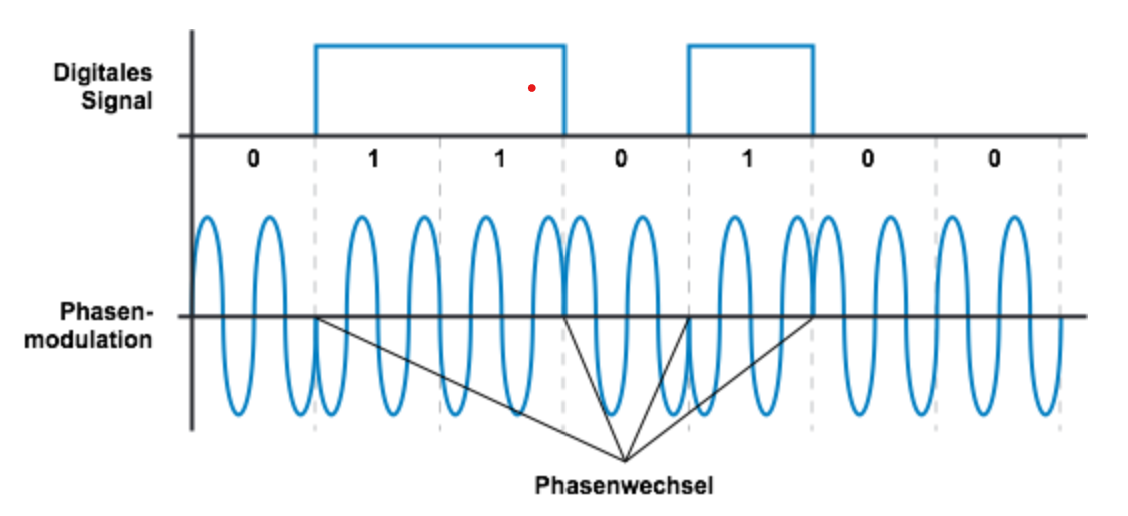
\includegraphics[width=0.5\textwidth]{Pictures/04020211.png}
    \caption{Phasenmodulation}
    \footnotesize{Quelle: \url{https://www.elektronik-kompendium.de/sites/kom/0402021.htm}}
\end{figure}

\section{Blockdiagramm einer Sendestrecke}
Im folgenden Abschnitt wird die Hochfrequenz-Übertragungsstrecke eines typischen Funksystems beschrieben. Bei der Grafik .. , handelt es sich um ein Blockdiagramm. Es zielt darauf ein grundlegendes
systematisches Verständinis aufzubauen um das gelernte auf unsere spezifische Hardware anwenden zu können. Die einzelnen Komponenten der Hochfrequenz-Übertragungsstrecke 
und deren Zusammenspiel wird im Anschluss näher erläutert und auf ihre Realiserung in unserer Hardware eingegangen.\\
\\Bild\\

\subsection{DAC}
Ein Digital-Analog-Wandler (eng. digital-to-analog converter, DAC) wandelt digitale Signale oder einzelne Werte in Analoge
Signale um. Bei einem digital Signal handelt es sich um ein zeit- und wertdiskretes Signal. Durch die Wandlung
in ein analoges Signal wird das Signal zeit- und wertkontinuierlich.  Dafür werden die Rechtecksignale des digitalen Eingangssignals mit Hilfe einer Fouriertransformation
in eine  kontinuirlich veränderliche Spannung transfomiert. Diese Wandlung ist erforderlich um das Signal über eine
Antenne aussenden zu können, da Antennen nur elektormagnetische Wellen abstrahlen können. \\

\subsection{LO und Mischer}
Der lokale Oszillaotr(eng. local oscillator, LO) erzeugt eine ungedämpfte hochfrequente Trägerschwingung. Diese Trägerschwingung 
wird benötigt, um das analoge Signal auf die gewünschte Frequenz zu bringen. Der LO kann in verschiedenen Frequenzen arbeiten,
abhängig von der Anwendung und dem gewünschten Frequenzbereich des Signals. Der Mischer übernimmt die Modulation des
Bandsignals auf eine Hochfrequenz. Dies geschieht durch die Multiplikation des Bandsignals mit der Trägerschwinung des LO.

\begin{equation}
    S_{xx}(t) \cdot S_{xx}(t) \rightarrow S_{xx}(t)
\end{equation}


\subsection{PA}
Der Leistungsverstärker (eng. power amplifier, PA) verstärkt das modulierte Signal auf eine Leistung, die für die Übertragung über eine Antenne 
geeignet ist. Die hohe Leistung ist notwedig um über eine größere Diszanz senden zu können und um Zuverlässigkeit und
Signalqualität zu gewährleisten. 

\subsection{Drahtlose Übertragung mit Antennen}
Die Sendeantenne strahlt das modulierte HF Signal Sxx als elektromagnetische Wellen in den Raum ab. DIese abgstrahlte Welle
breitet sich mit Lichtgeschwindigkeit aus und kann von Empfängerantennen empfangen werden. Die Empfängerantenne wandelt
die elektromagnetische welle wieder in eine elektrische Spannung um, die dann weiterverarbeitet werden kann. Diese entspricht
jedoch nicht mehr dem ursprünglichen Bandsignal, da es durch die Übertragungseinflüsse wie Dämpfung, Rauschen und Interferenzen
und vielen weiteren Einflüssen gedämpft und gestört wurde.

\subsection{LNA}
Bei dem LNA (eng. low noise amplifier) handelt es sich um einen rauscharmen HF-Verstärker. Das empfangene Signal Sxx ist
durch die bereits erwähnten Einflüsse sehr schwach und muss  zuerst verstärkt werden, um weiterverarbeitet werden. Daher
ist eine Verstärkung des Signals unmittlbar nach der Antennen zwingend notwendig. Der Vorteil des LNA gegenüber zu
anderen Verstärkern ist, dass er kein nennenswertes Rauschen hiinzufügt. Dies ist wichtig, da jedes zusätzliche Rauschen
die folgende Demolution erheblich erschweren würde. Ebenfall ist durch die Postion des LNA das empfangene Signal noch 
nicht durch andere elektrischen Komponenten verfälscht worden, was durch eine spätere Verstärkung zu rekonstruktionsproblemen
des eigentlichen Signals führen könnte.
\subsection{Demodulation}
Iwas mit Nyquisr Theorem und Abtastrate 

\subsection{ADC}
Nun muss das demodulisierte Signal wieder in ein digitales Signal umgewandelt werden, damit es weiterverarbeitet werden kann.
In unsere Schaltung wird dafür ... verwendet. 


\section{Mathematische Grundlagen: Fourier-Transformation}
\subsection{Betrag und zeitlicher Verlauf von Rechteckfunktion}
Der Rechteckimpuls ist eine wichtige Funktion in der Signalverarbeitung.
Er wird häufig in der Kommunikationstechnik verwendet, um digitale Signale zu repräsentieren.
Der Verlauf der Rechteckfunktion $x(t)$ ist in Abbildung \ref{fig:rechteck} dargestellt.
\begin{figure}[H]
    \centering
    \begin{tikzpicture}
        \begin{axis}[
            width=0.8\textwidth,
            height=5cm,
            axis lines=middle,
            xlabel={$t$},
            ylabel={$x(t)$},
            domain=-2:2,
            samples=200,
            xtick={-2,-1,0,1,2},
            ytick={0,1},
            ymin=-0.2, ymax=1.2,
            grid=both,
        ]
        % Null-Linie links
        \addplot[blue, thick, samples=2, domain=-2:-1] {0};
        % Rechteck oben
        \addplot[blue, thick, samples=2, domain=-1:1] {1};
        % Null-Linie rechts
        \addplot[blue, thick, samples=2, domain=1:2] {0};
        % Vertikale Linie bei t=-1
        \addplot[blue, thick, samples=2, domain=0:1] ({-1},{x});
        % Vertikale Linie bei t=1
        \addplot[blue, thick, samples=2, domain=0:1] ({1},{x});
        \end{axis}
    \end{tikzpicture}
    \caption{Verlauf der Rechteckfunktion $x(t)$ mit Amplitude 1 im Intervall $-1 < t < 1$}
    \label{fig:rechteck}
\end{figure}

Die Fourier-Transformierte der Rechteckfunktion $x(t)$ ist gegeben durch:
Die Fourier-Transformierte einer Rechteckfunktion der Breite $2T$ und Höhe $1$ ist die normierte $\mathrm{sinc}$-Funktion:
\[
\mathcal{F}\{x(t)\} = 2T \cdot \mathrm{sinc}(T\omega) = 2T \cdot \frac{\sin(T\omega)}{T\omega}
\]
Der Verlauf (inklusive Vorzeichen) der Fourier-Transformierten ist in folgender Abbildung dargestellt:

\begin{figure}[H]
    \centering
    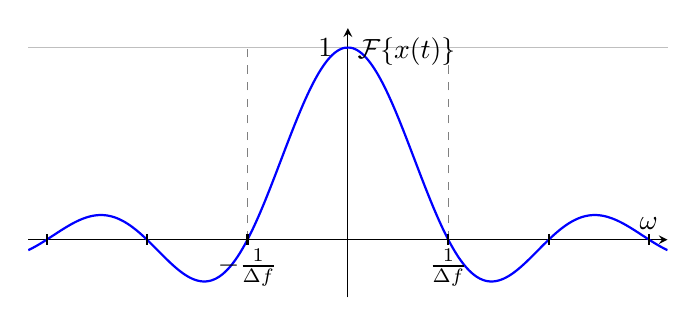
\begin{tikzpicture}
        \begin{axis} [
            width=0.8\textwidth,
            height=5cm,
            axis lines=middle,
            xlabel={$\omega$},
            ylabel={$\mathcal{F}\{x(t)\}$},
            domain=-10:10,
            samples=400,
            xtick=\empty, % entfernt die Zahlen auf der x-Achse
            ytick={-1,0,1},
            ymin=-0.3, ymax=1.1,
            grid=both,
        ]
        \addplot[blue, thick, samples=400, domain=-10:10] {sin(deg(x))/x};
        % Markiere die Nullstellen bei x = -pi und x = pi (entspricht ±1/Δf)
        \draw[dashed,gray] (axis cs:-3.1416,0) -- (axis cs:-3.1416,1);
        \draw[dashed,gray] (axis cs:3.1416,0) -- (axis cs:3.1416,1);
        \node[below] at (axis cs:-3.1416,0) {$-\frac{1}{\Delta f}$};
        \node[below] at (axis cs:3.1416,0) {$\frac{1}{\Delta f}$};
        % Einfache Striche für Vielfache von 1/Delta f
        \foreach \k in {-3,-2,-1,1,2,3} {
            \addplot[black, thick, mark=none, domain=0:0.03, samples=2] coordinates {({\k*3.1416},0.03) ({\k*3.1416},-0.03)};
        }
        % Optional: Nullstelle bei 0 markieren (falls gewünscht)
        % \addplot[black, thick, mark=none, domain=0:0.03, samples=2] coordinates {(0,0.03) (0,-0.03)};
        \end{axis}
    \end{tikzpicture}
    \caption{Verlauf der Fourier-Transformierten der Rechteckfunktion: $\mathrm{sinc}(\omega)$, Nullstellen bei Vielfachen von $\frac{1}{\Delta f}$}
    \label{fig:fourier_rechteck}
\end{figure}

\subsection{Betrag und zeitlicher Verlauf von Sinusfunktion}
Der Sinus ist eine wichtige Funktion in der Signalverarbeitung.
Er beschreibt eine harmonische Schwingung und ist in der Fourier-Analyse von Bedeutung. Sein Verlauf ist in der Abbildung \ref{fig:sinus} dargestellt.
Die Sinusfunktion $x(t) = \sin(t)$ hat eine Periode von $2\pi$ und schwingt zwischen -1 und 1. Sie ist symmetrisch um die $y$-Achse, was bedeutet, dass $x(-t) = -x(t)$ gilt. Dies ist eine Eigenschaft der ungeraden Funktion.

\begin{figure}[H]
    \centering
    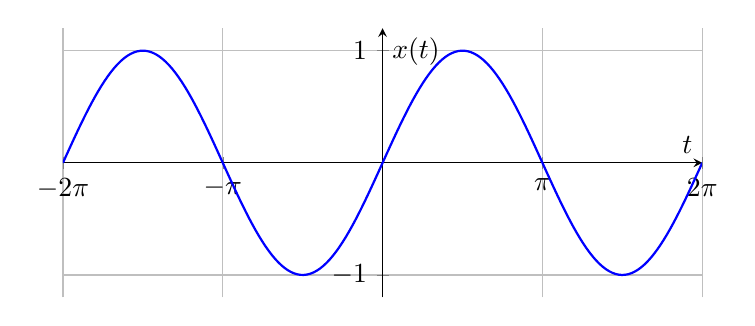
\begin{tikzpicture}
        \begin{axis}[
            width=0.8\textwidth,
            height=5cm,
            axis lines=middle,
            xlabel={$t$},
            ylabel={$x(t)$},
            domain=-2*pi:2*pi,
            samples=200,
            xtick={-6.2832,-3.1416,0,3.1416,6.2832},
            xticklabels={$-2\pi$,$-\pi$,$0$,$\pi$,$2\pi$},
            ytick={-1,0,1},
            ymin=-1.2, ymax=1.2,
            grid=both,
        ]
        \addplot[blue, thick] {sin(deg(x))};
        \end{axis}
    \end{tikzpicture}
    \caption{Verlauf der Sinusfunktion $x(t) = \sin(t)$ über zwei Perioden symmetrisch um die $y$-Achse}
    \label{fig:sinus}
\end{figure}

Seine Fourier-Transformierte sieht wie folgt aus:
Die Fourier-Transformierte der Sinusfunktion $x(t) = \sin(t)$ ist gegeben durch:
\[
\mathcal{F}\{\sin(\omega_0 t)\} = \pi j \left[ \delta(\omega + \omega_0) - \delta(\omega - \omega_0) \right]
\]
Für $\omega_0 = 1$ ergibt sich:
\[
\mathcal{F}\{\sin(t)\} = \pi j \left[ \delta(\omega + 1) - \delta(\omega - 1) \right]
\]
Der Betrag der Fourier-Transformierten besteht aus zwei Dirac-Impulsen bei $\omega = \pm 1$.
\begin{figure}[H]
    \centering
    \begin{tikzpicture}
        \begin{axis}[
            width=0.8\textwidth,
            height=5cm,
            axis lines=middle,
            xlabel={$\omega$},
            ylabel={$\mathcal{F}\{\sin(\omega_0 t)\}$},
            xtick={-1,0,1},
            xticklabels={$-\omega_0$,$0$,$\omega_0$},
            ytick=\empty,
            ymin=-1.2, ymax=1.2,
            xmin=-1.5, xmax=1.5,
            grid=both,
            clip=false,
        ]
        % Dirac impulses: +1 at -omega0, -1 at +omega0
        \addplot+[ycomb, thick, blue, mark=*, samples at={-1}] {1};
        \addplot+[ycomb, thick, red, mark=*, samples at={1}] {-1};
        \node[above] at (axis cs:-1,1) {$\pi j\,\delta(\omega + \omega_0)$};
        \node[below] at (axis cs:1,-1) {$-\pi j\,\delta(\omega - \omega_0)$};
        \end{axis}
    \end{tikzpicture}
    \caption{Graphische Darstellung von $\pi j [\delta(\omega + \omega_0) - \delta(\omega - \omega_0)]$ für $\omega_0=1$}
    \label{fig:fourier_sinus_komplex}
\end{figure}

\subsection{Multiplikation der beiden Funktionen im Zeitbereich}


\section{Zusammenhang von Datenrate und Bandbreite}
blabla
\clearpage